\documentclass[letterpaper,twocolumn,openany,nodeprecatedcode]{dndbook}

% Use babel or polyglossia to automatically redefine macros for terms
% Armor Class, Level, etc...
% Default output is in English; captions are located in lib/dndstrings.sty.
% If no captions exist for a language, English will be used.
%1. To load a language with babel:
%	\usepackage[<lang>]{babel}
%2. To load a language with polyglossia:
%	\usepackage{polyglossia}
%	\setdefaultlanguage{<lang>}
\usepackage[english]{babel}
%\usepackage[italian]{babel}
% For further options (multilanguage documents, hypenations, language environments...)
% please refer to babel/polyglossia's documentation.

\usepackage[utf8]{inputenc}
\usepackage[singlelinecheck=false]{caption}
\usepackage{lipsum}
\usepackage{listings}
\usepackage{shortvrb}
\usepackage{stfloats}
\usepackage{hyperref}

\captionsetup[table]{labelformat=empty,font={sf,sc,bf,},skip=0pt}

\MakeShortVerb{|}

\lstset{%
  basicstyle=\ttfamily,
  language=[LaTeX]{TeX},
  breaklines=true,
}

\title{Organization}
\author{}
\date{}

\begin{document}

% \frontmatter

% \maketitle

% \tableofcontents

% \mainmatter%

\footnotesize

\begingroup
\DndSetThemeColor[PhbMauve]

\section{Warfare}

% The system we presented in \textit{Strongholds \& Followers} didn’t make a whole lot of sense! You could have 8 infantry units who were all somehow able to attack a single enemy unit without in any way needing to coordinate their movements.

% only worked if everyone played along, and it didn’t make a lot of sense. As long as everyone was playing in the spirit of things, it worked fine. But as soon as folks started using it competitively, it broke down. Players could decide not to activate their units, and the entire battle ground to a halt.

% Also

% Finally, it

% The current system is now essentially its own game. This was necessary to create a system that was robust enough to support the ways people were using it.

We assume Battles happen rarely. Once per adventure usually. And usually in the final battle, where we expect things to get a little hairy. So using this system shouldn’t be burdensome for those rare scenarios.

But this system is straightforward enough that running a battle, in which each player usually only commands a handful of units, should be pretty easy! And fun!

\subsection{Battlefield}

The biggest change is the fact that the \textbf{battlefield} now has a shape.
Figure \ref{fig:battlefield} shows the battlefield your war will happen on. The rules assume \textbf{two sides}.
% (there may be options for more, but this is the default and covers most use cases).

\begin{figure*}
    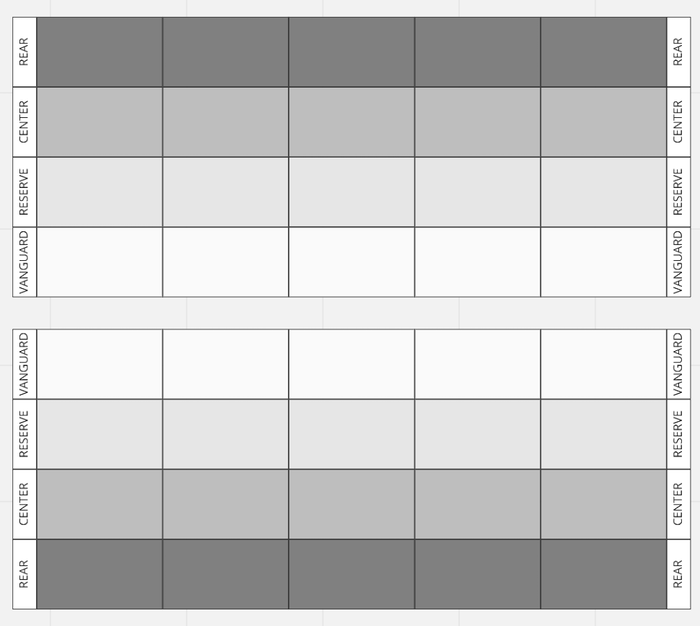
\includegraphics[width=\textwidth]{battlefield.pdf}
    \caption{The Battlefield layout.}
    \label{fig:battlefield}
\end{figure*}

% As soon as you see this you think “Oh god,” because obviously now instead of an abstract system we’re talking about a game. But in fact I think all these rules make things easier because now units have a position and movement and it’s obvious where everything is and moving and attacking is simple.

\begin{DndReadAloud}
    Explaining "Who Can Attack Who" in the old system was weird and complex and hard to hold in your head while you were doing everything else. By using a battlefield, constrained to a specific shape with units moving from one square to another, now Warfare works the same way every other game in the world does and that makes things a lot more straightforward.
\end{DndReadAloud}

% \textbf{Let’s break down this battlefield.}

Each side has four \textbf{Ranks}. Your Infantry deploy either in your \textbf{Vanguard}, \textbf{Rear}, or \textbf{Reserves}. Your artillery (including archers and siege weapons) deploy in your \textbf{Center}. Once the battle starts your units can move wherever they want.
% :D

Units can move one space forward, backward, left or right. They cannot move diagonally. Infantry can attack any adjacent unit along these cardinal directions. Artillery and Aerial units can attack \textbf{anyone}.

Cavalry and Aerial units belong to no rank. However, Cavalry units can only attack infantry or artillery if they are \textbf{exposed}, meaning there’s no other units between your target and the edge of the battlefield.
% for which there are rules in the system. Basically, if
% , your cavalry can attack them.
% Imagine the cavalry riding around the battlefield, looking for openings, smashing into any unprotected infantry.

The exception is the \textbf{Center} and the \textbf{Reserves} which are protected from Cavalry and not exposed as long as there are units in your Rear \textbf{and} your Front. Your Front is your Vanguard and the entire enemy side.

To visualize place Cavalry and Aerial unit cards in your enemies \textbf{Flank}. For quick reference use table \ref{tab:warfare:battlefield}.

\begin{table}
    \begin{DndTable}[]{XX}
        \textbf{Rank} & \textbf{Unit Types} \\
        Vanguard    & Infantry \\
        Reserves    & Infantry \\
        Center      & Artillery \\
        Rear        & Infantry \\
        Flank (None)& Cavalry, Aerial \\
    \end{DndTable}
    \caption{Battlefield positions and Unit Types.}
    \label{tab:warfare:battlefield}
\end{table}

So while you may want to ignore your rear and focus on your vanguard, if your enemy has cavalry, you’ll need to put some units in your rear or your archers will get steamrolled. Maybe some levies in the rear to buy time for your archers, or maybe some pikemen with Set For Charge, who can make sure any Cavalry attacking them get a rude surprise.

% That’s it. That’s the entire order of battle. I’ve now run this system dozens of times for friends and folks at MCDM, the testers have run it even more. We’ve all found it fun and easy to learn. Let’s look at a unit!

\subsection{Units}

\begin{figure}
  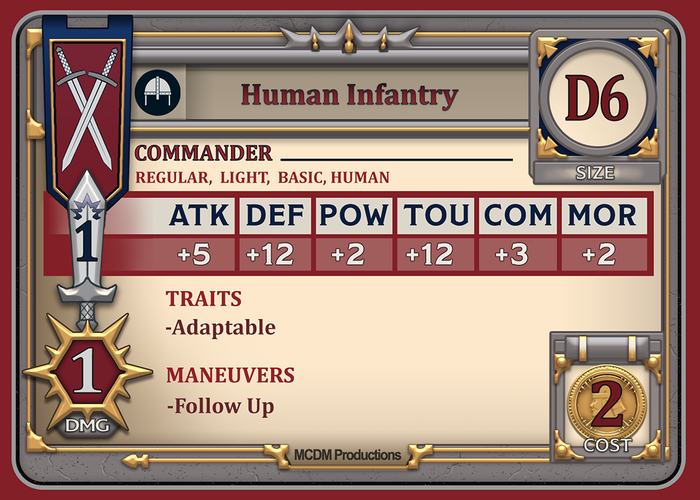
\includegraphics[width=\linewidth]{images/Human Infantry.png}
  \caption{Human Infantry}
  \label{fig:human_inf}
\end{figure}

Figure \ref{fig:human_inf}, \ref{fig:elf_art}, and \ref{fig:hobgoblin_inf} show unit cards.
%You can see there's a space on the card to write down which character (a PC presumably) "owns" or commands the unit.
The stats are (from left to right): \textbf{Attack}, \textbf{Defense}, \textbf{Power}, \textbf{Toughness}, \textbf{Command}, \textbf{Morale}. The sword represents how many attacks the unit gets, and the star below it, how much damage it does on a successful power test.

\subsubsection{Equipment \& Experience}

This is a basic human unit, you can improve it by buying \textit{better equipment} for it, so it goes from \textbf{Light} to \textbf{Medium}, to \textbf{Heavy} or \textbf{Super-heavy}. And it can \textit{level up by winning battles}, going from \textbf{Regular} to \textbf{Veteran} to \textbf{Elite} and then \textbf{Super-elite}.

A unit like this is easy to recruit by building a Stronghold or making an Operations check during Intrigue. But each ancestry also has Special units the DM can award though good roleplaying and inventive use of your Domain skills.
% Like the Hounds of Dalrath!

% \begin{figure}
%   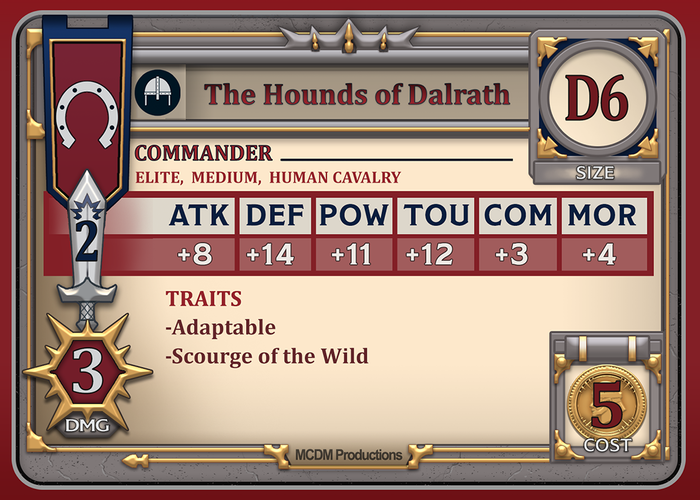
\includegraphics[width=\linewidth]{images/The Hounds of Dalrath.png}
%   \caption{The Hounds of Dalrath}
%   \label{fig:hounds_of_dalrath}
% \end{figure}

% Look at these guys! Two attacks! (The sword icon.) Three damage on a successful power test! And they have SCOURGE OF THE WILD.

% \textbf{Scourge of the Wild: This unit has +2 attack vs Orcs, Goblinoids, and Elves.}

% These guys are going to ruin someone's day. And, of course, we have other ancestries!

\subsubsection{Ancestries}

% Six ancestries: Humans and Orcs, Elves and Dwarves, Goblins and Undead.

Figure \ref{fig:human_inf} is a typical human infantry unit.

All \textbf{human} units get the Adaptable trait.

\textbf{Adaptable: This unit has advantage on Morale and Command tests.}

\begin{figure}
  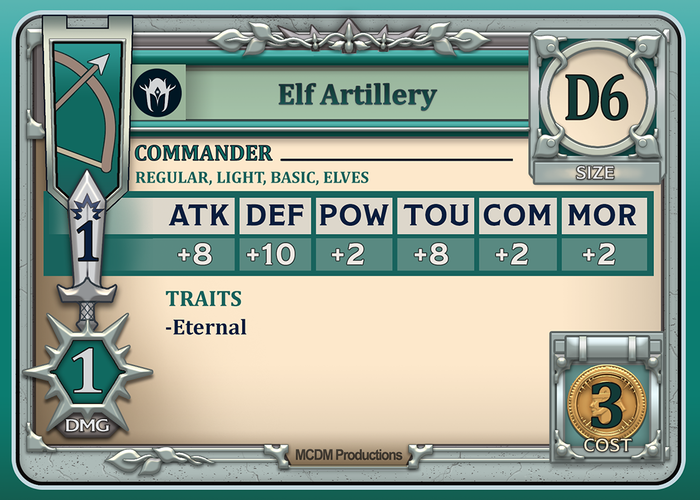
\includegraphics[width=\linewidth]{images/Elf Artillery.png}
  \caption{Elf Artillery}
  \label{fig:elf_art}
\end{figure}

% I think Jason did a killer job with these unit cards.

Figure \ref{fig:elf_art} is a basic Elf unit you can recruit if you're an Elf, or if your Domain is allied with the elves. Or you might fight these guys in battle if the Enemy Realm is a Fae Court!

\textbf{Elves} get the Eternal trait.

\textbf{Eternal: This unit has advantage on morale tests vs Undead and Infernal Units}

% They also have Forest as their favored terrain which means they get to be good archers even though they’re in a forest with trees blocking line of sight.

But what does an enemy unit look like? Take a look at Figure \ref{fig:hobgoblin_inf}.

\begin{figure}
  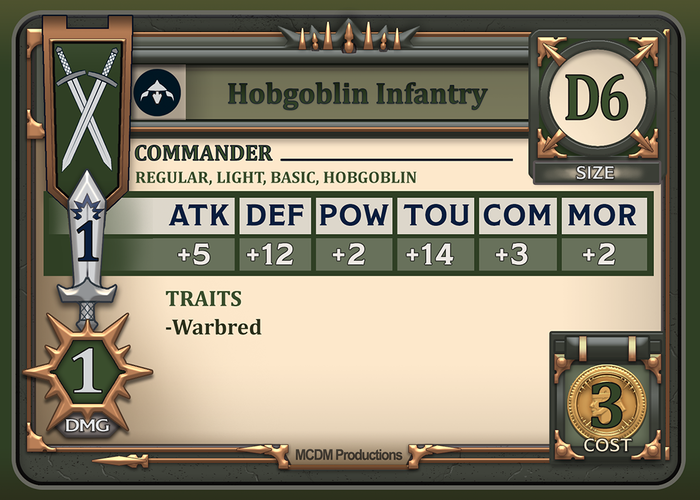
\includegraphics[width=\linewidth]{images/Hobgoblin Infantry.png}
  \caption{Hobgoblin Infantry}
  \label{fig:hobgoblin_inf}
\end{figure}

Hobgoblins! All hobgoblins are Warbred.

\textbf{Warbred: This unit has advantage on attack tests.}

\begin{DndReadAloud}
That seems really good. If the design is successful, “Adaptable” won’t seem like a super exciting ability compared to Warbred, but then you play it and you realize that advantage on Morale and Command is basically “You are good at War.” So humans have this low-key ability that just makes them better at warfare in a way other species find annoying.
\end{DndReadAloud}

\subsubsection{Unit Types}

\paragraph{Infantry} have low attack and power, but high defenses.

\paragraph{Artillery} have high attack, average power, and low defenses.

\paragraph{Cavalry} have average attack and defenses, but high power and inflict \textbf{two} casualties on a successful power test. Cav can only attack exposed units, but they hit \textbf{hard}.

\paragraph{Aerial} units combine the best of all of the above!

\subsubsection{Command \& Maneuvers}

\textbf{Command} represents how well trained your army is and whether it can execute complex commands, called \textbf{Maneuvers}.

\textbf{Maneuvers} are special actions your units can take instead of attacking. All infantry units, for instance, have the \textbf{Follow Up} maneuver.

\textbf{Follow Up: As a reaction to an enemy unit adjacent to this unit breaking or moving out of its space, make a DC 8 Command test. If successful, move into that space.}

% We have ... I dunno how many, over 50 different units already designed. The final product will probably have over 100. Six ancestries are currently supported with a full array of Basic and Special units. Units for Humans and Orcs, Elves and Dwarves, Goblins and Undead. Along with rules for levelling them up and buying them better equipment.

% Then there’s another 50 or so Unique covering lots of monsters and other ancestries like Minotaurs or Kobolds. But nothing crazy, no Iron Golems for instance. The general rule for this design is; if it’s a monster your players would want to fight? Then you face it in the Combat. Otherwise it’s legal to be a Special Unit.

% \begin{DndReadAloud}
% If you’re familiar with the Warfare system in Strongholds \& Followers, you may not notice an immediate difference here, but let’s go over the whole thing.
% \end{DndReadAloud}

\subsubsection{Attacking}

\begin{DndReadAloud}
Folks were ok with the two-roll system, but they \textit{didn’t} like the fact that they might pass on an attack roll, fail their power test and therefore “nothing happened.”
\end{DndReadAloud}

When you attack another unit, you make a d20 \textbf{Attack} roll against the enemy unit’s \textbf{Defense}. If that roll passes, \textbf{you inflict one casualty} and move on to the Power Test.

Your infantry successfully executed your Attack order, but how strong are they? Are they physically strong enough, is their gear good enough, to really hurt the enemy unit? That’s the \textbf{Power} test, another d20 roll vs the enemy’s \textbf{Toughness}. If this test passes, you inflict casualties equal to the \textbf{damage} rating of the unit, which is \textit{usually 1}.

\subsubsection{Morale}

When a unit is reduced to \textbf{half its starting size} (usually 3 casualties) it has to make a \textbf{Morale} test or suffer another casualty. This only happens once for each unit. Morale is also a measure of how your army reacts to things like Battle Magic.

\subsubsection{Rally}

Casualties mean deaths, but also the idea that some of the soldiers in this unit might be confused, or disoriented, not know exactly who to attack or even which direction the enemy is. Some soldiers might run screaming from the battle. So there are a few ways to \textbf{Rally} a unit and regain a few casualties in battle.

\subsection{Victory and Defeat}

% There are more rules than this obviously ... but not many!
At the beginning of each turn, if a rank has no units in it, it collapses and the ranks that were in front and behind become adjacent. The battlefield shrinks over time as the armies close in on each other.
% This helps keep infantry relevant since they don’t have to march as far to reach the enemy as the battle progresses.

\begin{DndReadAloud}
The final rules will also cover the \textbf{Tide of Battle} where the combat between the heroes and the villain will affect the armies they command, and the armies clashing can affect the combat between the characters. This creates dynamic synergies between the two and make it feel like the combat and the battle are all part of one big conflict. Also, I just unironically used the phrase “dynamic synergies” but dammit it’s the proper term for this!
% I stand by my decision.
\end{DndReadAloud}

At the end of every turn, after all units have activated, you check to see if one side has twice as many points left as the other. If not, you keep fighting! If so, whoever has the larger army has won and the enemy must \textbf{Retreat} (a maneuver that determines whether you suffer any more casualties getting your units to safety) so they can live to fight another day.

You might \textit{wish} your units would suicide themselves (undead units would obviously be ok with this if they are sufficiently mindless) but their commanders are not being mind controlled and will not recklessly waste the lives of their soldiers.

That’s it! I mean that’s ... that’s most of the rules!
% We have already used these rules a lot and played lots of battles and even when we were just using the basic units, Infantry, Cavalry, Artillery, no maneuvers or battle magic or special units, it was fun. It was a lot of fun! Jason, our art director, quickly realized the potential of the Follow Up maneuver and used it to set traps for my infantry! And I fell for it! Once… :D

% We imagine the default way folks will use Warfare will be \textit{during} the Final Battle of an adventure. You play one round of Combat, then stop and play one round of Warfare. Each character usually only controls a handful of units, three would be a lot for your first battle.

% So while it may seem like a lot, having three units move and make a handful of rolls is pretty easy and it happens \textit{fast}. And it provides just a \textit{ton} of fantastic opportunities for the players and the GM to narrate events, a resounding clash of arms!

% Like the Domain system, this system won’t be for everyone. I’ve played some \textit{fantastic} miniature wargames that would be great for handling epic battles like we imagine happening in our campaigns, but none of them are simple enough to use \textit{during} a 5E game.

% You may find this system is too much, it’s too extra. I respect that. But for me, and hopefully some of you, this is \textit{exactly} what I want for my games. It can be used as its own system, or dropped in the final battle, or deployed whenever the adventure calls for it. The battle for a bridge across a gaping chasm! The battle for control of a city as the units fight over each neighborhood!

% If you want to watch me and Jason, our Art Director, actually playing this system, you can see it in this Twitch Stream.

% https://www.twitch.tv/videos/746124131?t=0h11m13s

% It's me, live, going over a pre-recorded video of me and Jason using Warfare. We ran a lot of battles, but I only recorded two: one with just basic units and no maneuvers or battle magic, then another one WITH some maneuvers and battle magic and even the simplest battle was fun!

% The system has been refined further, mostly just tweaking stats, but you get a good sense of it in that livestream.

% Anyway I hope you like it. I’ve worked ... \textit{incredibly} hard on this and I’m excited as hell. I think these two systems, either together or apart, can \textbf{really} change the kinds of games GMs can run.

% There’s still a lot of \textit{writing} left to do, as well as testing, but the core design is now finished. All that’s left is iteration.

\begin{DndComment}{So far so good.}
    For now I will try to adjust the units from Strongholds \& Followers, so that we can play with these new rules.
    So we will focus on the rules above. But keep reading if your are interesting in whats to come.
    Later I will hopefully have a robust idea on how to homebrew battle magic.
\end{DndComment}

% \pagebreak

\subsection{Martial Training \& Battle Magic}

Each class gets access to six different abilities, including new traits and maneuvers they train their soldiers in, and special items they can create and distribute in Warfare. They unlock these at a rate of one every other level, starting with one maneuver or item at first level.

If you compare these first three Sorcerer abilities with the three Barbarian abilities, they should all be straightforward and thematic. The Barbarian’s abilities affect all their light infantry, their special abilities last throughout the entire battle and make them better fighters.

Whereas the Sorcerer’s battle magic is more devastating (a Scroll of Firestorm can \textbf{vaporize} an entire unit!) but are one-use. Flashier, more damaging, but limited use.

% We have 78 such abilities already designed and in various states of testing, including 6 abilities for the Illrigger!

\subsubsection{Barbarian}

So your 5th-level Barbarian PC has the following three Martial Training abilities:

\textbf{Furious Assault.} Your Light Infantry gain +1 movement and inflict +1 damage on a successful attack test.

\textbf{Mobility Training.} Your light infantry can automatically Follow Up and may immediately make an attack against an adjacent enemy unit when they do.

\textbf{Berserkers.} Your infantry automatically pass at morale tests to become diminished. Your diminished infantry have advantage on Power tests.

% I think, if all you know is what I’ve described in this update, you should be able to figure out what these abilities do and why they’re cool. :D
The idea is, your Barbarian trained the units you control. The units are just regular soldiers, a Barbarian’s units aren’t “all barbarians” but because they were trained by a Barbarian, they fight like Barbarians.

If we’ve done a good job with these, they should reinforce the core fantasy of the Barbarian. Barbarians favor light armor, melee combat, they like being highly mobile and they get really pissy once they’ve suffered a few casualties.

They’re so bad-ass, they (almost uniquely in the game so far) inflict bonus damage on the \textbf{Attack} test!

% We’ve run a bunch of battles with these maneuvers and it’s pretty breathtaking when the Barbarian player goes and activates their Light Infantry and they just chew their way across the battlefield. It is appropriately barbariany. :D

\subsubsection{Sorcerer}

But what if there’s a 5th-level Sorcerer commanding a handful of artillery? Well, unlike a martial class that sorcerer doesn’t spend a lot of time training their troops, that’s not what a spellcaster is about. Instead, they craft special items they hand out to the sergeants commanding their units, like:

\textbf{Wand of Fire.} Target an enemy unit, which must pass a DC 15 Power test or suffer 1 casualty and gain a fire token.

\textbf{Scroll of Mass Invisibility.} Choose a number of allied units equal to your command rating. They become Hidden (enemy units attacking hidden units have disadvantage on attack and power tests) until their next activation.

\textbf{Scroll of Firestorm.} Choose an enemy unit. It must pass a DC 15 Power test or suffer 1d4+2 casualties. If it passes it suffers 2 casualties.

These items are \textbf{temporary} and lose their magic at the end of the battle, which helps keep your campaign from exploding with wands and scrolls.

Each item is unique. \textbf{Wands} can be used every round and must be distributed to Artillery or Aerial units. \textbf{Scrolls} are one-use and we don’t know which unit has which scroll until they use it.
% The drone flying over the battlefield is too far away, the individual soldiers too small to tell which sergeant has which scroll. But once they use it, you can tell!

\subsubsection{Battlemagic}

% It’s worth nothing,
\textbf{Any time an enemy unit is affected by Battle Magic, it must make a Morale Test.} On a failed test the unit takes 1 casualty. The common soldiers, who were maybe only recently peasants, don’t like magic, it freaks them out. More experienced soldiers are sophisticated and have higher morale. They know what to expect once spells start slinging.

\chapter{Homebrew}

\section{TL;DR}

\subsection{Positions}

\paragraph{Adjacent}

Units can move one space forward, backward, left or right.
They cannot move diagonally.
Infantry can attack any \textbf{adjacent} unit along these cardinal directions.

\subsection{Command Rating}

Your character has a \textit{command rating} equal to either your \textbf{organisations level} or your \textbf{stronghold level},
which ever is higher.
If your character has neither a stronghold nor an organisation, it is \textbf{1 (one)}.

\subsection{Conditions}

% \paragraph{Burning} (Fire Token)
% A burning unit

\paragraph{Frightened}
A frightened unit has disadvantage on ability and attack tests while the source of its fear is on the battlefield.
% or adjacent as in "line of sight" not cardinal directions for movement or attack

\paragraph{Hidden}
Enemy units attacking hidden units have disadvantage on attack and power tests.

\paragraph{Leaderless}
A leaderless unit has disadvantage on Command and Morale tests.

\paragraph{Poisoned}
A poisoned unit has disadvantage on Attack and Power tests.
% Must repeat the save or take one casualty.
% Once passed the unit is no longer poisoned.

\subsection{General Maneuvers}

\paragraph{Follow Up}
\textit{Infantry}

As a reaction to an enemy unit adjacent to this unit breaking or moving out of its space, make a DC 8 Command test.
If successful, move into that space.

\paragraph{Rally}
\textit{any unit}

Any unit that would be removed from battle can be rallied.
Their commander makes a DC 15 Morale test.
On a success, the unit remains in the battle with its casualty die at 1, but it cannot be rallied again.
On a failure, the unit is removed from battle.

\paragraph{Retreat}
\textit{any unit}

%You can only give this order when all of your side’s units are fresh.

All of your units immediately make a Morale test (DC 15) and are removed from the battle, ending the battle.
The retreating army suffers any consequences of defeat and the normal penalties for failing the Morale check made to retreat.

\section{Martial Training \& Battle Magic}

Characters get access to \textbf{Special Actions} and \textbf{Traits} based on their class.
Martial classes mostly use \textbf{Maneuvers}.
While spellcasters get access to \textbf{Battle Magic} in the form of \textbf{Wands} and \textbf{Scrolls}.

\subsection{Types of Features}

\paragraph{Trait} Passive feature that is always active.
\paragraph{Maneuver} Can be used every turn.
\paragraph{Wand} Can be used every turn.
\paragraph{Scroll} Can be used once per battle.

\subsection{Class Features}

\subsubsection{Druid}

\paragraph{Staff of Shillelagh}
\textit{Trait}.

Your Light Infantry gain +1 Power and +1 Damage.
% old
% When your Light Infantry attacks an enemy unit,
% they gain +1 Power and +1 Damage.

\paragraph{Scroll of Spike Growth}
\textit{Scroll}. (shared with ranger)

Choose an enemy unit.
It must pass a DC 15 Power test or suffer 1d4 casualties
and can not move during its next turn.
% Either way it

\paragraph{Scroll of Healing Spirit}
\textit{Scroll}. (shared with ranger)

Choose one of your units.
Every allied unit adjacent to it, including itself,
regain a number of casualties equal to your command rating.

\paragraph{Scroll of Moonbeam}
\textit{Scroll}.

Choose an enemy unit.
It must pass a DC 15 Power test or suffer 1d4+2 casualties.
If it passes it suffers 2 casualties.

\paragraph{Scroll of Woodland Beings}
\textit{Scroll}.

You summon a unit of woodland beings.
If the summoned unit is non-aerial,
choose a free space for the unit to appear in.
Either within in your \textbf{Ranks}
or adjacent to one of your units.
% TODO: special woodland units

% wild shape (maybe not, maybe special unit)
\paragraph{Scroll of Feral Strength}
\textit{Scroll}.

As a bonus action, choose a Light Infantry unit.
They gain a bonus of +2 Power and +3 Damage until their next activation.


\subsubsection{Fighter}

% The Fighter should have the best maneuvers. Either the most complex, strong or general.

% things fighters are good at:
% - heavy equip
% - multi attack
% - maneuvers
% - command

\paragraph{Armor Expert}
\textit{Trait}.

Your heavy units gain +1 command and +1 power.

\paragraph{Engage}
\textit{Maneuver}.

As a bonus action, choose a number of allied units equal to your command rating.
They gain either +1 movement or +1 attack until the end of their next activation.

\paragraph{Retaliate}
\textit{Maneuver}.

As a reaction to an allied unit getting attacked,
adjacent units can make a DC 10 command test,
if they passes they inflict a casualty.

\paragraph{Volley}
\textit{Maneuver}.

Choose an Artillery unit and a number of enemy units equal to your command rating.
Your unit attacks the enemy units.
If they hit, they get advantage on the Power test.

\paragraph{Charge}
\textit{Maneuver}.

Choose a Cavalry unit and an enemy \textbf{Rank}, which is exposed.
The unit charges through said Rank.
Any unit within the Rank needs to pass a DC 15 Morale test or suffer 2 casualties.

\paragraph{Switch}
\textit{Maneuver}.

Choose two units that are adjacent to one another.
The two units switch places.
Each enemy unit chosen that passes a DC 10 Power test can resist.

\subsubsection{Rogue}

\paragraph{Sneak Attack}
\textit{Trait}.

If your unit is \textbf{Hidden} and attacks they gain +1 Power and +1 Damage.

% ambush
\paragraph{Stealth Mission}
\textit{Maneuver}.

As a bonus action, choose an allied unit with Light Equipment.
They become \textbf{Hidden} until their next activation.
While they are \textbf{Hidden} they may attack from the flank like cavalry.
% maybe they just move to the flank?
% or are allowed to move there?
% or if the do so, they are "stuck" there, being a target to any unit

\paragraph{Bandits}
\textit{Trait}.

When an enemy unit disperses and your Infantry uses Follow Up,
they loot the equipment and gain +1 power or +1 defense.
Each unit can only benefit from each bonus once.

\paragraph{Marksmen}
\textit{Maneuver}.

Choose a Artillery unit.
They attack with advantage and inflict 1 more casualty on a successful power test.

\paragraph{Assassination}
\textit{Maneuver}.

Target an enemy unit.
It must pass a DC 15 Power test or become leaderless.

% FIXME: make it a dot instead of a condition
\paragraph{Poison}
\textit{Maneuver}.

Target an enemy unit.
It must pass a DC 15 Power test or become poisoned.

\paragraph{Dust of Disappearance}
\textit{Scroll}.

Choose a number of allied units equal to your command rating.
They become \textbf{Hidden} until their next activation.

\subsubsection{Warlock}

\paragraph{Armor of Agathys}
\textit{Trait}.

Whenever one of your units gets attacked by Infantry or Cavalry.
The attacking unit must pass a DC 10 Power test
or suffer a number of casualties equal to your command rating.

\paragraph{Scroll of Mass Invisibility}
\textit{Scroll}.

Choose a number of allied units equal to your command rating.
They become \textbf{Hidden} until their next activation.

\paragraph{Scroll of Hadar}
\textit{Scroll}.

Choose an allied unit.
Every enemy unit adjacent to it need to pass a DC 15 Power test or suffer 1d4 casualties.

\paragraph{Scroll of Hex}
\textit{Scroll}.

Choose an enemy unit.
This unit is now cursed.
Any unit attacking it gains +1 Power and +1 Damage.

Choose an ability (Attack, Power, Command or Morale).
The cursed unit has disadvantage on test made with that ability.
If the target passes a test with that ability anyway,
it can make a DC 15 Power test to end the curse.

\paragraph{Eldritch Wand}
\textit{Wand}.

Target an enemy unit, which must pass a DC 15 Power test or suffer 2 casualty.

\paragraph{Scroll of Fear}
\textit{Scroll}.

Choose an enemy unit.
It must pass a DC 15 Morale test or be frightened by one allied unit of your choice.

\paragraph{Scroll of Confusion}
\textit{Scroll}.

Choose an enemy unit.
The unit must pass a DC 15 Power test, or be confused.

\begin{table}
    \begin{DndTable}[header=Confusion]{lX}
        \textbf{d10} & \textbf{Behavior} \\
        1 & The unit move in a random direction and does not take an action. \\
        2-6 & The unit doesn't move or take actions this turn. \\
        7-8 & The unit uses its action to attack a randomly determined unit within its reach. \\
        9-10 & The unit can act and move normally. \\
    \end{DndTable}
\end{table}


\end{document}
